
%\documentclass[a4paper]{jarticle}

\section{mglmnet.rb elastic net正則化による一般化線形モデル\label{sect:mglmnet}}
\index{mglmnet@mglmnet}
本コマンドは、統計パッケージRで提供されているglmnet
(\url{http://cran.r-project.org/web/packages/glmnet/index.html})
を利用しやすいように作成されたコマンドで、
elastic net正則化による一般化線形モデルを構築する。
本コマンドの特徴は以下の通りである。

\begin{itemize}
 \item Rスクリプトを書かなくても利用できる。
 \item 入力データとしてCSVで表現された疎行列を扱う。
 \item 正則化として、L1正則化(LASSO)、L2正則化(リッジ回帰)、およびL1とL2の中間的位置づけのelastic-net正則化が利用できる。
 \item 線形回帰、ポアソン回帰、ロジスティック回帰、多項ロジスティック回帰を扱うことができる。
 \item 交差検証により推定エラー最小のlambdaを決定することで最適モデルを構築可
 \item 回帰モデルの構築モードと未知データを与えての予測モードがある。
\end{itemize}

近年の情報収集技術の発展に伴い、データの規模はサンプル数のみならず変数の次元においても拡大の一途をたどっている。
DNAのマイクロアレイデータや工場のラインに設置された大量のセンサーデータ、文書分類に用いる単語ベクトルなどはその典型である。
さらに、高い関連性を持つアイテムの組み合わせ列挙やグラフ構造マイニングにおけるクリーク列挙など、
データマイニングの諸技術が生成するパターンは、時に膨大な数に達する。
これらのデータの特徴は、変数の数$p$がサンプル数$n$よりも多くなることにある。
例えば、新聞記事の内容分類について考えると、我々の経験によると、サンプル数は多くても数千のオーダである一方で、
単純なbug-of-wordアプローチであっても、その単語数は数千〜数万にも及び、
さらに格フレームなど単語の組み合わせを考慮に入れると、時にその数は数百万のオーダとなることも珍しくない。
このような大規模な数の変数から有用な変数を選択し回帰モデルを構築するには、
最小二乗法による回帰係数の推定およびAICに代表される変数選択といった従来の方法では対処できず、
そのような中から出てきたのが、正則化(regularization)を用いた回帰モデルにおける変数選択の諸手法である。

%解の不定性により係数を一意に推定できない。
%従来の回帰分析で用いられる変数選択においては、与えられた変数の全ての組み合わせの中から、
%部分的に(時には全て)ように、回帰係数の推定には最小二乗法を、そして変数選択にAICを
%が一般的に用いられるが、
%する必要性が増しており、

%回帰モデルにおける回帰係数の推定には最小二乗法が一般的に用いられてきたが、
%この方法だと、変数の数が増えれば増えるほど目的関数である二乗誤差を低減させることになり、
%訓練データに過度に適合したモデルが構築されてしまう。
%そこで、修正済み決定係数やAICに代表されるように、変数の数をペナルティとした評価基準によって変数の選択が行われる。
%変数の数が少ない場合は、全ての変数の組合せについて評価することで最適なモデルを得ることが可能である。

目的変数$y$および説明変数ベクトル$\ve x$についての回帰モデルについて考えると、
正則化による係数ベクトル$\ve w$は式\ref{eq:glmnet_problem}によって推定される。

\begin{equation}
\hat {\ve w}=\argmin_{\ve w} \frac{1}{n}\ell(y_i,{\ve w}^{\T}{\ve x}_i)+\lambda \Omega({\ve w})
\label{eq:glmnet_problem}
\end{equation}

ここで$\ell$は推定の悪さを評価するロス関数で、$\Omega({\ve w})$がモデルの複雑さを評価する正則化項で、
全体としてモデルの精度と複雑さのトレードオフを評価する式となっている。
ここで$\lambda$は、トレードオフをチューニングするパラメータで、
$lambda$を大きくすればする正則化それらの重みを
ロス関数は想定するモデルによって異なるが、線形回帰モデルの場合は、
モデルの予測値と実測値の平均二乗誤差が用いられる。
そして正則化項として

\begin{equation}
\hat {\ve w}=\argmin_{\ve w} \frac{1}{n} \sum (y_i-{\ve w}^{\T}{\ve x})^2 + \lambda ||{\ve w}||_1
\label{eq:glmnet_problem}
\end{equation}

%このような評価基準は、誤差最小化と変数の数に基づくペナルティという意味でL0正則化と呼ばれる方法である。
%しかし、L0正則化では、変数の全ての組み合わせ探索となるために
またそれが現実的でなければ、グリーディな探索によってある程度の満足解が得られる。
しかしながら、変数の数$p$が膨大な数になった場合、

正則化とは、パラメータ推定および変数選択において、および回帰モデルにおける
列挙を中心としたデータマイニングの諸手法が出力する膨大な数のパターンから、
目的変数に寄与するパターン(変数)を選択可能とする正則化は有用な方法である。
%文書分類モデルの構築において、文書に含まれる単語を特徴ベクトル(feature vectors)と考え、
%文書内容の分類モデルを回帰モデルによって構築するケースを考えると、
%一般的には、文書数(サンプル数)より特徴数(独立変数)の方が多くなる。
%また遺伝子解析においても、遺伝子の数に比べてサンプル数が少ない
%正則化による回帰モデルの構築は、
本コマンドは、統計パッケージRで提供されているglmnet
(\url{http://cran.r-project.org/web/packages/glmnet/index.html})
を利用しやすいように作成されたコマンドで、
以下の様な特徴を持つ。

本コマンドが直接扱うデータ構造は、
表\ref{tbl:mglmnet_inp1}に示されるような、サンプルID(tid)と説明変数名(item)、
およびそれらの値(val)を一行とした形式(以下、疎行列形式CSVと呼ぶ)のデータである。
一般的な回帰分析のツールが扱う行列形式のデータに変換すると表\ref{tbl:mglmnet_inp2}のようになるが、このデータ形式は本コマンドでは扱わない。

また目的変数は別ファイルとしてサンプルIDとその値のペアとして表\ref{tbl:mglmnet_inp3}のように与える。
なお、目的変数のデータ型は、想定するモデルによって異なるが、表\ref{tbl:mglmnet_inp3}では、線形回帰モデルを想定している。
説明変数と目的変数のデータはtid項目によってサンプルが紐付けられていることを前提としており、
一方に存在しないサンプルIDがあれば、そのIDは内部で削除されることになるので注意する。

以上のデータセットについて回帰分析を実行するには、
以下のようにコマンドを実行すればよい。
基本的にはファイルの指定とモデルのタイプ(\verb|family|)を指定するだけでよい。
結果として、表\ref{tbl:mglmnet_out}に示されるように、いくつかの結果データが出力される。

\begin{verbatim}
$ mglmnet.rb i=tra.csv c=profit.csv O=results family=gaussian
\end{verbatim}


\begin{table}[htbp]
\begin{center}
\begin{tabular}{ll}

\begin{minipage}{0.3\hsize}
\begin{center}
\caption{疎行列形式による説明変数データ。
顧客購買データで考えると、顧客ID(tid)と購入商品(item)および数量(val)と考えればよい。\label{tbl:mglmnet_inp1}}
{\small
\begin{tabular}{ccc}
\hline
tid&item&val\\
\hline
t1&a&1\\
t1&c&2\\
t1&d&1\\
t1&e&3\\
t2&a&1\\
t2&e&1\\
t3&b&1\\
t3&d&1\\
t3&e&2\\
t4&a&1\\
t4&c&4\\
\hline
\end{tabular} 
}
\end{center}
\end{minipage}

\begin{minipage}{0.3\hsize}
\begin{center}
\caption{表\ref{tbl:mglmnet_inp1}を行列形式に変換した場合のデータ。
本コマンドでは、この形式のデータは扱わない。\label{tbl:mglmnet_inp2}}
{\small
\begin{tabular}{cccccc}
\hline
tid&a&b&c&d&e \\
\hline
t1&1&0&2&1&3\\
t2&1&0&0&0&1\\
t3&0&1&0&1&1\\
t4&1&0&4&0&0\\
\hline
\end{tabular} 
}
\end{center}
\end{minipage}

\begin{minipage}{0.3\hsize}
\begin{center}
\caption{目的変数のデータ例。
顧客購買データで考えると、顧客別の年間粗利金額と考えればよい。\label{tbl:mglmnet_inp3}}
{\small
\begin{tabular}{cr}
\hline
tid&profit \\
\hline
t1&10 \\
t2&-20 \\
t3&23 \\
t4&0 \\
\hline
\end{tabular} 
}
\end{center}
\end{minipage}

\end{tabular} 
\end{center}
\end{table} 

\begin{table}[htbp]
\begin{center}
\begin{tabular}{ll}

\begin{minipage}{1.0\hsize}
\begin{center}
\caption{本コマンドが出力するデータ一覧。
ファイル名がcv\_から始まるデータは、
-nocvオプションを指定した場合は出力されない。\label{tbl:mglmnet_out}}
{\small
\begin{tabular}{lll}
\hline
ファイル名&内容&例\\
\hline
\verb|model.robj|       & 回帰モデルのRオブジェクト(バイナリ)         & テキストでは表示できない。\\
\verb|model_info.csv|   & 回帰モデルに関する各種情報                  & 表\ref{tbl:mglmnet_model_info_csv} \\
\verb|coef.csv|         & lambda別係数一覧                            & 表\ref{tbl:mglmnet_coef_csv} \\
\verb|coef.png|         & lambda別係数チャート                        & 図\ref{fig:mglmnet_coef_png} \\
\verb|lambda_stats.csv| & lambda別の各種情報(deviance,係数が非0のfeature数、推定誤差など) & 表\ref{tbl:mglmnet_lambda_stats_csv} \\
\verb|lambda_error.png| & lambda別エラーチャート                      & 図\ref{fig:mglmnet_lambda_error_png} \\
\verb|map_item2vno.csv| & オリジナルitem文字列と内部の変数番号の対応表& 表\ref{tbl:mglmnet_map_item2vno_csv} \\
\verb|scp.R|            & 実行されたRスクリプト                       & 表\ref{tbl:mglmnet_scp_R} \\
\hline
\end{tabular} 
}
\end{center}
\end{minipage}

\end{tabular} 
\end{center}
\end{table} 

\begin{table}[htbp]
\begin{center}
\begin{tabular}{ll}

\begin{minipage}{0.5\hsize}
\begin{center}
\caption{coef.csv: 疎行列形式によるlambda別の係数データ。
item項目に値がないものは定数項を表している。
lambdaが14.28の場合、定数項が14.28で、説明変数の係数は全て0であるため、
この表には出力されていない。
同様に、lambdaが13.63の場合、説明変数aの係数のみ1.49でその他の係数は0である。
この表を行列形式に変換した表が表\ref{tbl:mglmnet_coef2}に示されている。
\label{tbl:mglmnet_coef_csv}}
{\small
\begin{tabular}{crr}
\hline
item&lambda&coef \\
\hline
    &14.28 & 1.75 \\
    &13.63 & 0.62 \\
a   &13.63 & 1.49 \\
    &13.01 &-0.44 \\
a   &13.01 & 2.93 \\
$\vdots$ & $\vdots$ & $\vdots$ \\
    &10.80 &-4.27 \\
a   &10.80 & 7.17 \\
c   &10.80 & 1.29 \\
$\vdots$ & $\vdots$ & $\vdots$ \\
    & 6.78 &-11.16 \\
a   & 6.78 &13.04 \\
b   & 6.78 &-0.014 \\
c   & 6.78 & 6.36 \\
e   & 6.78 &-0.059 \\
$\vdots$ & $\vdots$ & $\vdots$ \\
\hline
\end{tabular} 
}
\end{center}
\end{minipage}

\begin{minipage}{0.5\hsize}
\begin{center}
\caption{
表\ref{tbl:mglmnet_coef_csv}を行列形式で表現したももの。
この表は出力されないが、mcrossコマンドを用いれば簡単に作成できる。
\label{tbl:mglmnet_coef2}}
{\small
\begin{tabular}{rrrrrrr}
\hline
lambda&定数&a&b&c&d&e \\
\hline
  14.28 &   1.75 &   0    &   0    &   0    &   0    &   0     \\
  13.63 &   0.62 &   1.49 &   0    &   0    &   0    &   0     \\
  13.01 &  -0.44 &   2.93 &   0    &   0    &   0    &   0     \\
$\vdots$&$\vdots$&$\vdots$&$\vdots$&$\vdots$&$\vdots$&$\vdots$ \\
  10.80 &  -4.27 &   7.17 &   0    &   1.29 &   0    &   0     \\
  10.31 &  -5.12 &   7.89 &   0    &   1.91 &   0    &   0     \\
$\vdots$&$\vdots$&$\vdots$&$\vdots$&$\vdots$&$\vdots$&$\vdots$ \\
   6.78 & -11.16 &  13.04 & -0.014 &   6.36 &   0    &  -0.059 \\
   6.48 & -11.20 &  13.44 & -0.060 &   6.53 &   0    &  -0.51  \\
$\vdots$&$\vdots$&$\vdots$&$\vdots$&$\vdots$&$\vdots$&$\vdots$ \\
\hline
\end{tabular} 
}
\end{center}
\end{minipage}

\end{tabular} 
\end{center}
\end{table} 



\begin{table}[htbp]
\begin{center}
\begin{tabular}{ll}

\begin{minipage}{0.5\hsize}
\begin{center}
\caption{lambda\_stats.csv: lambda別のモデル推定誤差。
dev.ratio:1.0-deviance/null deviance、cvm:交差検証による平均誤差、
cvsd:cvmの推定標準誤差、cvup:cvm+cvsd、cvlo:cvm-cvsd。
\label{tbl:mglmnet_lambda_stats_csv}}
{\small
\begin{tabular}{rrrrrr}
\hline
lambda&dev.ratio&cvm&cvsd&cvup&cvlo \\
\hline
14.28&0    &451.79&246.82&698.61&204.97 \\
13.63&0.071&449.02&248.04&697.06&200.97 \\
13.01&0.13 &444.82&248.98&693.81&195.83 \\
12.42&0.19 &437.71&249.08&686.80&188.62 \\
11.86&0.24 &431.41&249.11&680.53&182.30 \\
$\vdots$ & $\vdots$ & $\vdots$ \\
\hline
\end{tabular} 
}
\end{center}
\end{minipage}

\begin{minipage}{0.5\hsize}
\begin{center}
\caption{
model\_info.csv:構築されたモデルに関する各種統計を1行にまとめたもの。
nobs:サンプル数、lambdas:内部で利用されたlambdaの種類数、
nulldev:null deviance(定数項のみのモデルにおけるdeviance)、
lambda\_min:交差検証による最小誤差を達成したモデルのlambdaの値、
lambda\_1sd:交差検証による最小誤差+標準誤差を達成したモデルのlambdaの値。
\label{tbl:mglmnet_model_info_csv}}
{\small
\begin{tabular}{rrrrr}
\hline
nobs&lambdas&nulldev&lambda\_min&lambda\_1se \\
\hline
4&78&1016.75&0.39&6.78 \\
\hline
\end{tabular} 
}
\end{center}
\end{minipage}

\end{tabular} 
\end{center}
\end{table} 


\begin{figure}[htbp]
\begin{center}
\begin{tabular}{cc}

\begin{minipage}{0.5\hsize}
\begin{center}
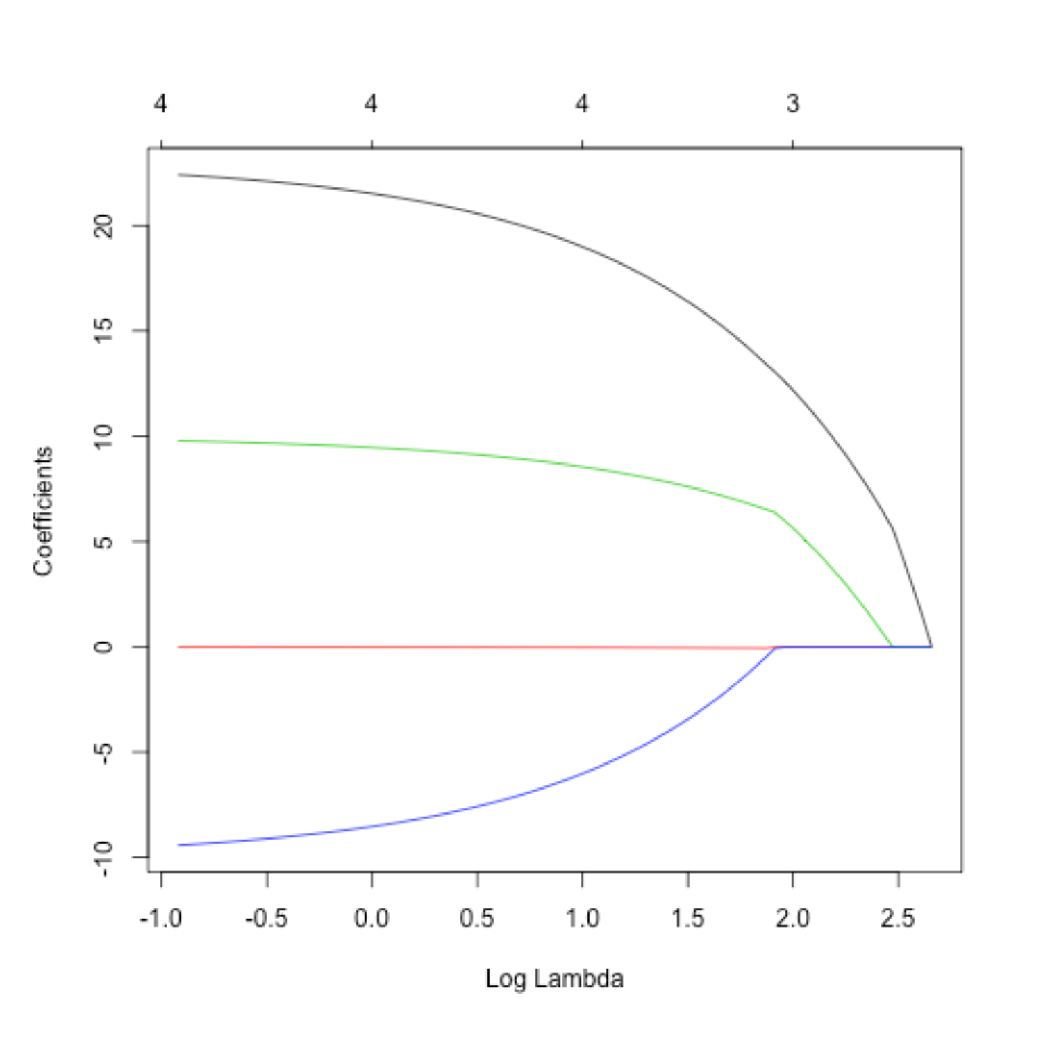
\includegraphics[scale=0.5]{./figure/coef.eps}
\caption{lambdaと係数の関係チャート。
このチャートは表\ref{tbl:mglmnet_coef_csv}を視覚化したものである。
一つの線が一つの変数の係数に対応しており、
対数化したlambdaとの関係が示されている。
\label{fig:mglmnet_coef_png}}
\end{center}
\end{minipage}

\begin{minipage}{0.5\hsize}
\begin{center}
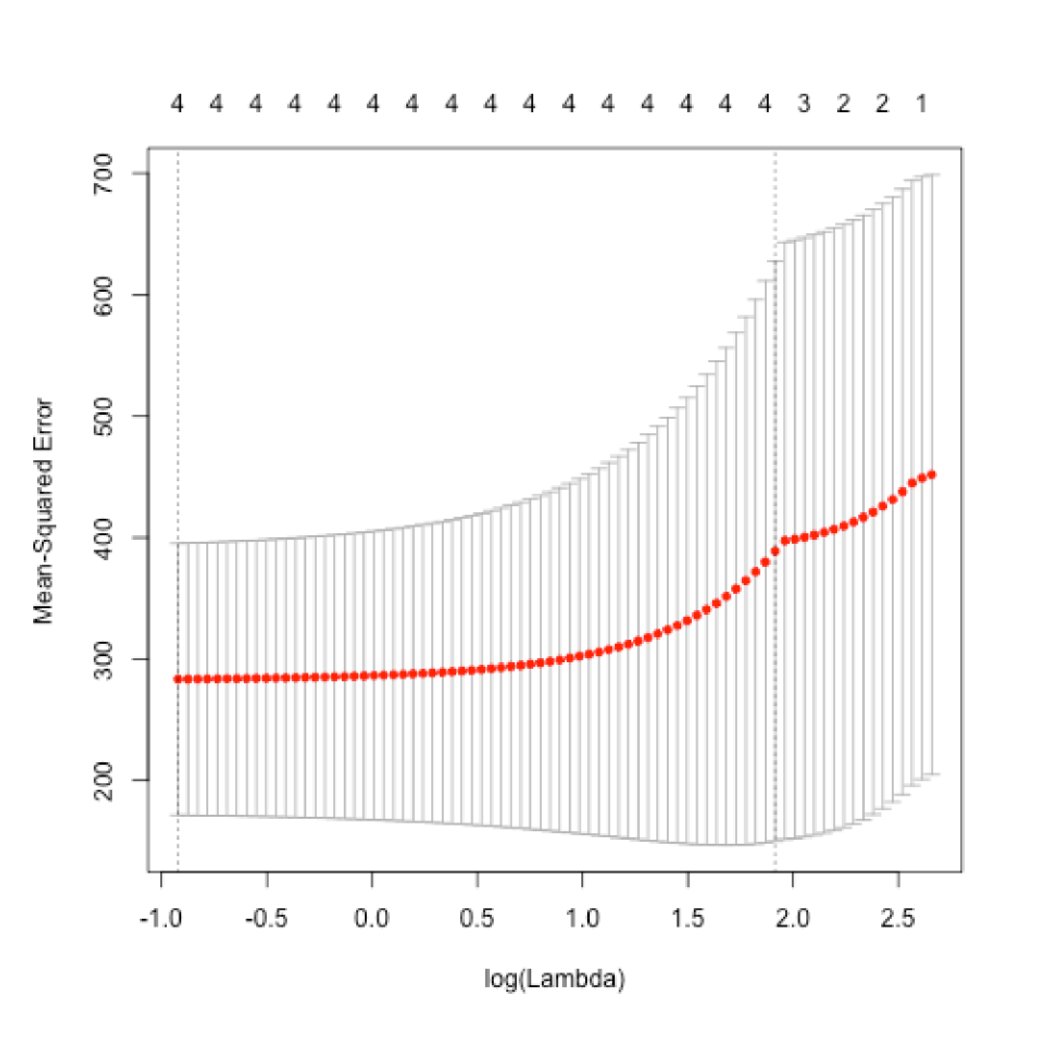
\includegraphics[scale=0.5]{./figure/lambda_error.eps}
\caption{lambdaとCVによるモデルの推定誤差の関係チャート。
表\ref{tbl:mglmnet_lambda_stats_csv}を視覚化したもので、
赤点が平均誤差(cvm)を、ヒゲがcvm±標準誤差(cvsd)の範囲を表している。
平均誤差最小値、および平均誤差最小値+標準誤差に対応するlamdaに点線が引かれている。
\label{fig:mglmnet_lambda_error_png}}
\end{center}
\end{minipage}

\end{tabular} 
\end{center}
\end{figure} 



\begin{table}[htbp]
\begin{center}
\begin{tabular}{ll}

\begin{minipage}{0.5\hsize}
\begin{center}
\caption{map\_item2vno.csv: 変数名(item)とRで扱う疎行列の列番号との対応表。
この表をユーザが直接利用することはないであろうが、
予測モード(-predict)において、与えられた未知データの変数名をこの表に従って番号に変換する。
\label{tbl:mglmnet_map_item2vno_csv}}
{\small
\begin{tabular}{cc}
\hline
vno&item \\
\hline
1&a \\
2&b \\
3&c \\
4&d \\
5&e \\
\hline
\end{tabular} 
}
\end{center}
\end{minipage}

\begin{minipage}{0.5\hsize}
\begin{center}
\caption{
内部で実行されるRスクリプト。
作業ディレクトリに格納された前処理データを入力データとして読み込んでいるため、
このスクリプトをRで直接実行しても動作しないことに注意する。
あくまでも、どのような処理がされているかの参考のために出力している。
\label{tbl:mglmnet_scp_R}}
{\scriptsize
\begin{Verbatim}[baselinestretch=0.7,frame=single]
#####################################
## setting csv data into a vector of objective valiable
yVEC= read.csv("/tmp/__MTEMP_17321_70142629480320_7",header=T)
yVEC = yVEC$class # as a vector
#####################################
## building a model with cross validation
model = cv.glmnet(xMTX,yVEC,family="gaussian",alpha=1.0)
fit=model$glmnet.fit
#####################################
## output serialized objects of the model
save(model ,file="result/model.robj")

#####################################
## output coefficients on each lambda
write.csv(as.matrix(fit$beta),file="/tmp/__MTEMP_17321_7014 ...
write.csv(as.matrix(fit$a0),file="/tmp/__MTEMP_17321_701426 ...

png("result/coef.png")
  plot(fit,"lambda")
dev.off()
                        :
\end{Verbatim}
}
\end{center}
\end{minipage}

\end{tabular} 
\end{center}
\end{table} 

\subsection{詳細}

分類モデルにおける目的変数を$y\in \{0,1\}$(0:負例,1:正例),
$p$個の説明変数(マイクロクラスタ)ベクトルを$\ve x=(x_1,x_2,\cdots,x_p)$とすると,
ロジスティック回帰モデルは式(\ref{eq:logistic})で表される.

\begin{align}
\label{eq:logistic}
\Pr(y=1 | \ve x) =
f \left(\ve \beta^{\T}\ve x + \beta_0\right)
\end{align}

$f(\cdot)$はロジスティック関数であり,
$f (a) =1/(1+\exp\left(-a\right))$で定義される.
%
$\ve \beta \in \mathbb R^{p}$, $\beta_0 \in \mathbb R$
は,それぞれ回帰係数ベクトルと定数項であり,
これらは訓練サンプルから推定するする.

回帰問題において$\ve \beta$の推定には最小2乗法を利用するのが一般的であるが,
説明変数の数$p$がサンプル数に比べて多いとき,
説明変数間の共線性が問題となり,異なる推定法が必要となる.
この問題に対して様々な推定法が提案されてきたが,
最小2乗法に$\ve \beta$に対する罰則を与えた上で最小化問題$\argmin\{||y-\ve \beta^{\T}\ve x||^2_2+J(\ve \beta)\}$($J(\ve \beta)$は罰則項)
を解く罰則付き回帰が有効であることがわかってきた.
その中でも$J(\ve \beta)=\lambda ||\ve \beta||_1$としたlasso,
および$J(\ve \beta)=\lambda ||\ve \beta||_2^2$としたridge回帰がよく利用される.
ここで,$||\ve \beta||_q$は$q$-ノルムで$||\ve \beta||_q=(\sum_{i=1}^{p} \beta_{i}^q)^{1/q}$である.
$\lambda \in [0,\infty)$は正の定数であり,
lassoにおいては$\ve \beta$をどの程度疎に選択するかのトレードオフパラメータである.
つまり$\lambda$が大きい場合には,$\ve \beta$の多くの値が$0$となる.
逆に$\lambda$が0の場合は通常の最小2乗法となる.
ridge回帰においては$\lambda$を,
大きく設定しても回帰係数が0と推定されることはないが,
推定値が全体的に小さく推定されることになる.

ridge回帰は共線性への対処法として用いられるが,変数選択としては機能しない.
一方でlassoは$\lambda$の値によっては多くの回帰係数が0となることから変数選択の有効な手法として注目されている.
しかしながら一方で共線性のある変数が選ばれにくいといった問題も指摘される.
%そこで,両者の罰則を按分し,$J(\ve \beta)=\lambda \{(1-\alpha)||\ve \beta||_2^2+\alpha||\ve \beta||_1\}$としたelastic netがある.
そこで,両者の罰則を結合し,$J(\ve \beta)=\lambda_1 |\ve \beta||_1 + \lambda_2||\ve \beta||_2^2$としたelastic netがある\cite{Zou05}.
本研究では,ridge回帰もlassoでも思ったようなモデル精度が得られなかったためにelastic netを使うことにした
\footnote{統計解析ツールRのパッケージglmnetを用いている.そこでは,$\lambda_1,\lambda_2$の調整を
$(1-\alpha)/2||\ve \beta||_2^2+\alpha||\ve \beta||_1 (0\le \alpha \le 1)$のように調整パラメータ$\alpha$によって実現している.
$\alpha$を0に近づければridge回帰の罰則が強くなり,逆に1.0に近づければlassoの罰則が優先される.
$\alpha$は試行錯誤の実験から0.001とした,}
%$\lambda$は10回の交差検証によりモデルの推定精度を最も高める値に定めた.
.

交差検証(CV)をしてもしなくても、複数のlambda値に対する回帰係数の推定は行われる。
      CVをすることで、lambda別に構築される回帰モデルの予測エラーを推定する。
      そして、エラー最小化という意味における最適なlambdaを得ることが可能となる。
      よって-nocvを指定した場合、CVによる予測エラーの推定を行わないため、
      予測モードにおいてlambda="min,1se"は指定できない。


\subsection{書式1:モデル構築モード}
\begin{verbatim}
       mglmnet.rb [family=] [alpha=] i= [tid=] [item=] [val=] c= [class=] O= [seed=] [-nocv]
                  [T=] [-mcmdenv] [--help]
\end{verbatim}

\begin{table}[htbp]
{\small
\begin{tabular}{ll}
\verb|i=|      & : 入力データ【必須】 \\
\verb|tid=|    & : 1つのサンプルを表す項目名【デフォルト:"tid"】 \\
\verb|item=|   & : 1つの変数を表す項目名【デフォルト:"item"】 \\
\verb|val=|    & : 説明変数の値項目【オプション】 \\
               & : 指定しなければ、全行1とする。 \\
\verb|c=|      & : 目的変数データファイル名【必須】 \\
\verb|class=|  & : 目的変数の項目名【デフォルト:"class"】 \\
               & : family=で指定した内容により以下に示す値である必要がある。 \\
               & :   gaussian: 実数 \\
               & :   poisson: 正の整数 \\
               & :   binomial: 2つのクラス値(文字列でも可) \\
               & :   multinomial: 複数クラス値(文字列でも可) \\
\verb|O=|      & : 出力ディレクトリ名【必須】 \\
\verb|family=| & : リンク関数【デフォルト:"gaussian"】 \\
               & : gaussian: 線形回帰 \\
               & : poisson: ポアソン回帰 \\
               & : binomial: ロジスティック回帰 \\
               & : multinomial: 多項ロジスティック回帰 \\
\verb|alpha=|  & : L1とL2正則化項の荷重【デフォルト:1.0】 \\
               & : 1.0でL1正則化、0でL2正則化、$0<alpha<1$でelastic-net正則化 \\
\verb|seed=|   & : 乱数の種(0以上の整数,交差検証に影響)【オプション:default=-1(時間依存)】 \\
\verb|-nocv|   & : 交差検証をしない \\
\verb|T=|      & : 作業ディレクトリ【デフォルト:"/tmp"】 \\
\verb|-mcmdenv|& : 内部のMCMDのコマンドメッセージを表示 \\
\verb|--help|  & : ヘルプの表示

\end{tabular} 
}
\end{table} 

\subsection{書式2:予測モード}

\begin{verbatim}
       mglmnet.rb -predict [lambda=] i= [tid=] [item=] [val=] I= o= [T=] [-mcmdenv] [--help]
\end{verbatim}

\begin{table}[htbp]
{\small
\begin{tabular}{ll}
\verb|i=|      & : 入力データ【必須】 \\
\verb|tid=|    & : 1つのサンプルを表す項目名【デフォルト:"tid"】 \\
\verb|item=|   & : 1つの変数を表す項目名【デフォルト:"item"】 \\
\verb|val=|    & : 説明変数の値項目【オプション】 \\
\verb|I=|      & : モデル構築モードでの出力先ディレクトリパス【必須】 \\
               & : 利用するファイルは以下のとおり。 \\
               & :   map\_item2vno.csv: データの変換に利用 \\
               & :   model.robj: 回帰モデルRオブジェクト  \\
\verb|lambda=| & : 正則化項の重み【必須:複数指定可】 \\
               & :   0以上の実数値を与える以外に、以下の2つは特殊な意味を持つシンボルとして指定できる \\
               & :   min: CVにおけるエラー最小モデルに対応するlambda \\
               & :   1se: lambda.min+1*standard errorのモデルに対応するlambda \\
\verb|o=|      & : 予測結果ファイル名 \\
               & :   tid,目的変数予測値... \\
               & : lambda=で指定した各lambdaに対応する予測値全てを出力する \\
\verb|T=|      & : 作業ディレクトリ【デフォルト:"/tmp"】 \\
\verb|-mcmdenv|& : 内部のMCMDのコマンドメッセージを表示 \\
\verb|--help|  & : ヘルプの表示

\end{tabular} 
}
\end{table} 


\subsection{利用例}
\subsubsection{例1 上記「解説」の例}
\begin{Verbatim}[baselinestretch=0.7,frame=single]
:
\end{Verbatim}

%\begin{thebibliography}{9}
%\bibitem{Bishop2008}
%C.M. ビショップ著, 元田浩, 栗田多喜夫, 樋口知之, 松本裕治, 村田昇(編), パターン認識と機械学習(下):ベイズ理論による統計的予測, 13章, pp.323--370, 2008.
%\end{thebibliography}

%\end{document}

